\documentclass[12pt]{article}
\usepackage[utf8]{inputenc}
\usepackage{amsmath, amssymb, amsthm}
\usepackage{enumitem}
\usepackage{geometry}
\usepackage{setspace}
\usepackage{graphicx}
\usepackage{hyperref}
\usepackage{tikz,tikz-cd}
\usepackage{float}
\usepackage{verbatim}

\usepackage{biblatex}
\addbibresource{references.bib}

\setstretch{1.25}
\geometry{
  letterpaper,
  lmargin=2cm,
  rmargin=2cm,
  tmargin=2.5cm,
  bmargin=2cm,
  footskip=12pt,
  headheight=12pt}
\renewcommand{\b}[1]{\textbf{#1}}
\newcommand{\eps}{\epsilon}
\newcommand{\R}{\mathbb{R}}
\newcommand{\Z}{\mathbb{Z}}
\newcommand{\Q}{\mathbb{Q}}
\newcommand{\C}{\mathbb{C}}
\newcommand{\E}{\mathcal{E}}
\renewcommand{\bar}[1]{\overline{#1}}
\renewcommand{\sl}{\mathfrak{sl}}
\newcommand{\xto}[1]{\xrightarrow{#1}}
\DeclareMathOperator{\Spec}{Spec}
\DeclareMathOperator{\Lie}{Lie}
\DeclareMathOperator{\rk}{rk}
\DeclareMathOperator{\coker}{coker}

\newtheorem{theorem}{Theorem}[section]
\newtheorem{corollary}[theorem]{Corollary}
\newtheorem{lemma}[theorem]{Lemma}

\newtheorem{proposition}[theorem]{Proposition}
\newtheorem{conjecture}[theorem]{Conjecture}

\theoremstyle{definition}
\newtheorem{definition}[theorem]{Definition}
\newtheorem{thm}[theorem]{Theorem}

\newtheorem{example}[theorem]{Example}

\theoremstyle{remark}
\newtheorem{remark}[theorem]{Remark}

\newcommand{\g}{\mathfrak{g}}
\renewcommand{\P}{\mathcal{P}}
\newcommand{\M}{\mathcal{M}}
\newcommand{\ch}{\mathrm{ch}}
\newcommand{\N}{\mathcal{N}}
\newcommand{\h}{\mathfrak{h}}
\DeclareMathOperator{\Hom}{Hom}
\newcommand{\cyc}{\mathrm{cyc}}
\newcommand{\gl}{\mathfrak{gl}}


\title{A formula for the $q$-character of functions on the nilpotent cone of some Lie algebra representations}
\author{Vasily Krylov and Frank Wang}

\begin{document}

\maketitle

\begin{abstract}
    Let $\g$ be a reductive Lie algebra and $V$ a finite-dimensional $\g$-representation. When $V$ is the representation of a cyclic quiver with equal dimensions, the representation of a cyclic quiver with two vertices, or a representation of a product of copies of $\sl_2$ we call an \emph{acyclic extended quiver representation of trivial type}, we prove a $q$-character formula for the nilpotent cone of $V$ analogous to Hesselink's $q$-character formula of the usual nilpotent cone of $\g$. We also define a new class of representations we call \emph{Hesselink-type representations}, for which we make a conjecture in relation to our formula and describe a geometric interpretation.
\end{abstract}

\section{Introduction}

Let $\g$ be a complex reductive Lie algebra and let $\N$ be its nilpotent cone. Then the ring of functions $\C[\N]$ has a natural grading via the usual degree of polynomials (coming from the degree of polynomials in $\C[\g]$), and one may consider the \emph{$q$-character} of $\C[\N]$, given by

\[\ch_q\C[\N]:=\sum_{d\geq 0}\ch(\C[\N]_d)q^d,\]
where $\C[\N]_d$ is the degree $d$ component of $\C[\N]$ and $\ch(\C[\N]_d)$ is the character of $\C[\N]_d$ as a $\g$-module. A well-known formula due to Hesselink \cite{hesselinkalg} for this $q$-character computes the multiplicity of an irreducible character in terms of a $q$-analog of the dimension of the zero weight space of the corresponding irreducible representation; see also \cite{mcgovern1989}, \cite[Proposition 4.0.1]{MasonBrown2022RegularFO}.

We will prove an analog of this formula for the nilpotent cone of a few classes of representations of Lie algebras. Namely, let $V$ be a finite dimensional representation of $G$, and let $\C[V]^G_+\subset\C[V]$ be the augmentation ideal of positive degree elements of $\C[V]^G$. Then one may define the \textbf{nilpotent cone of $V$} as $\N_V:=\Spec (\C[V]/\C[V]^G_+\C[V])$. Note that the $\C$-points of $\N_V$ are exactly the points $p$ such that the closure of the $G$-orbit of $p$ contains $0$. Then one may similarly define a grading on $\C[\N_V]$ coming from the usual grading on $\C[V]$, so we may consider $q$-characters in this setting as well. 

In this paper we will give a formula for the $q$-character of the nilpotent cone for some examples of representations. Specifically, we will consider the following examples:

\begin{enumerate}
    \item $V$ is the adjoint representation of $\g$.\label{eg:adj}
    \item Let $V_1,\dots,V_l$ be a collection of complex vector spaces of the same dimension $N$, and let $G=\prod_{k\in\Z/l\Z}GL(V_k),V=\bigoplus_{k\in\Z/l\Z}\Hom(V_k,V_{k+1})$. This is the representation of a cyclic quiver of length $l$ where the vector spaces assigned to each vertex have equal dimensions.\label{eg:eqdim}
    \item Let $V_1,V_2$ be complex vector spaces (of possibly different dimensions), and let $G=GL(V_1)\times GL(V_2),V=\Hom(V_1,V_2)\oplus\Hom(V_2,V_1)$. This is the representation of a cyclic quiver of length 2.
    \item Let $G$ be a product of finitely many copies of $SL_2(\C)$, and $V$ be one of the representations described in Section \ref{sec:sl2}.
\end{enumerate}

We will also give some examples of $q$-characters for other small representations as a starting point for creating a unified theory for $q$-characters of nilpotent cones for all representations.

Let us fix some notation. Fix a Cartan subalgebra $\h\subset\g$ and let $T\subset G$ be the torus with $\Lie T=\h$. Let $W$ be the Weyl group of $\g$ and $R$ be the root system of $\g$. Fix a set of positive roots $R_+$ and let $\rho=\frac{1}{2}\sum_{\alpha\in R_+}\alpha$, $\rho^\vee=\frac{1}{2}\sum_{\alpha\in R_+}\alpha^\vee$. Let $\Lambda$ be the weight lattice of $\g$ and let $\Lambda_+$ be the set of dominant weights. For $\lambda\in\Lambda_+$, let $L_\lambda$ be the irreducible representation of $\g$ with highest weight $\lambda$ and let $\chi_\lambda$ be its character. Let $\langle-,-\rangle$ be the natural pairing $\h\otimes\h^*\to\C$. For a graded vector space $Z$ we let $\dim_q Z:=\sum_{d\geq 0}\dim(Z_d)q^d$ be the graded dimension (or Hilbert series) of $Z$. 

Let $S$ be the multiset of the weights in $V$, and let 
\[S_+:=\{\alpha\in S\mid\langle\alpha,\rho^\vee\rangle>0\},\quad S_0:=\{\alpha\in S\mid\langle\alpha,\rho^\vee\rangle=0\},\quad S_-:=\{\alpha\in S\mid\langle\alpha,\rho^\vee\rangle<0\}\]
where each of $S_+,S_0,S_-$ is viewed as submultisets of $S$. Also, let $S_{\leq 0}:=S_-\cup S_0$. When we say a function on one of $S,S_+,S_0$, or $S_{\leq 0}$, we mean a function on all occurrences of weights in the multiset, not just on distinct weights.

Let $(S_0)_0$ be the set of all functions $m\colon S_0\to\Z_{\geq 0}$ such that $m\neq 0$ and $\sum_{\alpha\in S_0}m(\alpha)\alpha=0$. Let us call a function $m:S\to\Z_{\geq 0}$ \textbf{weakly negative} if $m(\alpha)=0$ for all $\alpha\in S_+$ and for all $m'\in (S_0)_0$, there is some $\alpha\in S_0$ such that $m(\alpha)<m'(\alpha)$. For a function defined on a sub(multi)set of $S$, we say it is \textbf{weakly negative} if its extension to $S$ by zero is weakly negative.

Consider the following $q$-analog of the Kostant partition function:
\[\P_q\colon\Lambda\to\Z[q],\]
\[
    \P_q(\mu)=\sum_{n=0}^\infty\#\Big\{m\colon S\to\Z_{\geq 0}\mid\sum_{\alpha\in S}m(\alpha)\alpha=-\mu,\sum_{\alpha\in S}m(\alpha)=n,\text{ $m$ is weakly negative}\Big\}q^n.
\]

A priori, this definition of $\P_q$ only lands in $\Z[[q]]$, but it in fact lands in $\Z[q]$ due to Dickson's lemma.

Note that when $V$ is the adjoint representation, $S_-$ is the set of negative roots $R_-$ and $S_0$ is a multiset of $\rk\,\g$ $0$'s, corresponding to $\h\subset\g$. In particular, $(S_0)_0$ is all nonzero functions $S_0\to\Z_{\geq 0}$, and a weakly negative function is simply a function $R_-\to\Z_{\geq 0}$. In this case $\P_q$ reduces to the $q$-analog of the Kostant partition function introduced by Lusztig \cite{lusztigqkostant}.

\begin{example}\label{eg:1,1}
    Consider the case of a cyclic quiver with two vertices that are both one-dimensional. Let $V_1,V_2$ be complex vector spaces with $\dim V_1=\dim V_2=1$. Then let $\g\subset\sl(V_1\oplus V_2)$ be the Lie algebra that fixes $V_1,V_2$, and let $V=\Hom(V_1,V_2)\oplus\Hom(V_2,V_1)$. Then we have $\g\cong\gl_1$, so we have $\rho^\vee=0$. The weight lattice $\Lambda$ is $\Z\subset\h^*\cong\C$, and $V$ has two weights which we can write as $\pm 1\in\Lambda$. Since $\rho^\vee=0$ we have $S=S_0=\{\pm 1\}$. So a weakly negative function is a function $m\colon\{\pm 1\}\to\Z_{\geq 0}$ such that either $m(1)=0$ or $m(-1)=0$. We thus obtain $\P_q(k)=q^{|k|}$ for any integer $k$. 
\end{example}

Also, define
\[\M_q\colon \Lambda\to\Z[q],\quad \M_q(\mu)=\sum_{w\in W}(-1)^{\ell(w)}\P_q(w(\mu+\rho)-\rho).\]

This is a $q$-analog of the Kostant multiplicity formula for the zero weight space of a representation that also generalizes the corresponding formula in \cite{lusztigqkostant}.

\begin{theorem}\label{thm}
    Let $G,V$ be one of the above cases. Then we have
    \[\ch_q\C[\N_V]=\sum_{\lambda\in\Lambda_+}\M_q(\lambda)\chi_\lambda.\]
\end{theorem}

Note that in case \ref{eg:adj}, $\N_V$ is the usual nilpotent cone of $\g$, and we recover the classical result of Hesselink described earlier for the $q$-character of functions on the nilpotent cone. 

We expect that there are more representations for which this formula holds, and it would be interesting to classify all such representations.

\begin{example}\label{eg:1,1N}
    Let us revisit the case of Example \ref{eg:1,1}. If $v_+,v_-$ are basis vectors of $\Hom(V_1,V_2)^*$, $\Hom(V_2,V_1)^*$, respectively, then $\C[V]^G=\C[v_+v_-]$, and we have $\C[\N_V]=\C[v_+,v_-]/(v_+v_-)$. Choose an isomorphism $\h^*\cong\C$ so that $v_+$ is the vector of weight $1$ and $v_-$ is the vector of weight $-1$. Since $R$ is empty, all weights are dominant. We have $W=1$, so $\M_q(k)=\P_q(k)$ and Theorem \ref{thm} reads
    \[\ch_q\C[\N_V]=\sum_{k\in\Z}q^{|k|}\chi_k.\]
    Indeed, for nonnegative $k$ the unique copy of $\chi_k$ in $\C[\N_V]$ is spanned by $v_+^k$ in degree $k$, and the unique copy of $\chi_{-k}$ in $\C[\N_V]$ is spanned by $v_-^k$ in degree $k$.

    Technically, Theorem \ref{thm} only considers the case where we take $\g$ to be the subspace of $\gl(V_1\oplus V_2)$ that fixes $V_1,V_2$ rather than $\sl(V_1\oplus V_2)$, but the theorem carries over to the latter since the copy of $\C$ in $\gl(V_1\oplus V_2)\cong\sl(V_1\oplus V_2)\oplus\C$ acts by zero on $V$. This also holds for all cyclic quivers.
\end{example}

\begin{remark}
    Outside the classes of representations encompassed by Theorem \ref{thm}, we also found similar-looking formulas for $\ch_q\C[\N_V]$ for some other representations $V$, which are described in Section \ref{sec:nonexamples}. We suspect there may be a more general formula for the $q$-character of the nilpotent cone for a broader class of representations, which we would be very interested in but were unable to find.
\end{remark}

For a finite dimensional $G$-representation $V$, let $V^{\rho^\vee}$ be the invariants in $V$ under the action of $\rho^\vee\in\h$. In other words, $V^{\rho^\vee}$ is the direct sum of all weight spaces in $V$ whose weights belong to $S_0$. Monomials in $\C[V^{\rho^\vee}]$ correspond to functions $S_0\to\Z_{\geq 0}$, monomials in $\C[V^{\rho^\vee}]^\h$ correspond to functions in $(S_0)_0$, and monomials surviving in $\C[V^{\rho^\vee}]/\C[V^{\rho^\vee}]^\h_+\C[V^{\rho^\vee}]$ are exactly the ones corresponding to weakly negative functions on $S_0$. Then we introduce the following new class of $G$-representations, motivated by the proof of Theorem \ref{thm}.

\begin{definition}\label{def:hesselink}
    A \textbf{Hesselink-type} representation is a representation $V$ such that
    \[X_V:=\frac{\sum_{w\in W}(-1)^{\ell(w)}t^{w\rho}\prod_{\alpha\in S_+}(1-qt^{-w\alpha})}{\sum_{w\in W}(-1)^{\ell(w)}t^{w\rho}}\]
    is a $\Z[q]$-multiple of the trivial character.
\end{definition}

In the process of proving Theorem \ref{thm}, we will show that all representations encompassed by the theorem are Hesselink-type.

A finite dimensional $G$-representation $V$ is called \textbf{cofree} if $\C[V]$ is free over $\C[V]^G$ (see \cite{book}, Chapter 8.1). Note that all representations covered in Theorem \ref{thm} are cofree; the adjoint representation is cofree by Kostant's theorem, and all representations of cyclic quivers are cofree as they fall under the class of $\Z/l\Z$-graded Lie algebras, and all such representations are cofree (\cite{vinberg}, \cite{book}). For the case $\g=\prod\sl_2$, we prove cofreeness directly in Section \ref{sec:sl2}. We will further elaborate on this point when we discuss these cases directly in Sections \ref{sec:eqdim} and \ref{sec:2vertex}.

We make the following conjecture, connecting Hesselink-type representations, cofree representations, and Theorem \ref{thm}.

\begin{conjecture}\label{conj:cofree}
    Let $G$ be semisimple. If $V$ is a Hesselink-type representation, then $V$ is cofree. Moreover, \eqref{eq:id} and Theorem \ref{thm} hold for $V$.
\end{conjecture}

\subsection{Motivation}

This paper was originally motivated by $D$-modules on the cyclic quiver and their relation to representations of the rational Cherednik algebra. Namely, let $V$ be the representation of a cyclic quiver with equal dimensions as in Case \ref{eg:eqdim} of Theorem \ref{thm} and let $D^G(V)$ be the category of $G$-equivariant $D$-modules on $V$. Consider the group $G(l,1,N):=(\Z/l\Z)^N\rtimes S_N$ and let $t,c,d_1,\dots,d_l$ be complex numbers. Then one has the \emph{rational Cherednik algebra} $H_{t,c,d}(G(l,1,N))$ (see \cite{rationalcherednik}), and in \cite{montarani} Montarani produced a functor $F_{N,\chi}:D^G(V)\to\text{Rep}\,H_{t,c,d}(G(l,1,N))$. Through this functor one may study graded characters of $H_{t,c,d}(G(l,1,N))$-modules by studying the $q$-characters of equivariant $D$-modules on $V$. 

The simplest case of an equivariant $D$-module on $V$ is the space of global functions $\C[V]$. In this case the $q$-character of $\C[V]$ as an equivariant $D$-module is exactly the $q$-character of $\C[V]$ as described above, and a formula for $\ch_q\C[V]$ is equivalent to a formula for $\ch_q\C[\N_V]$ via Lemma \ref{lem:cofreeiso}. We first derived the formula in Theorem \ref{thm} for this case, and after discussions with Pavel Etingof and Zhiwei Yun we realized it would be natural to consider generalizations of this formula for other groups and representations. 

In particular, much of this paper is a result of an attempt to generalize our formula to the $q$-character of the nilpotent cone of a $\Z/l\Z$ graded Lie algebra, following the work of Lusztig-Yun and others on graded Lie algebras (\cite{wille},\cite{LUSZTIG1995147},\cite{lusztigyun}). More explicitly, if $\tilde{\g}=\bigoplus_{i\in\Z/l\Z}\g_i$ is a graded Lie algebra with $[\g_i,\g_j]\subset\g_{i+j}$ and $\tilde{\N}$ is the nilpotent cone of $\tilde{\g}$, then the nilpotent cone of $\g_i$ is defined as $\N_i:=\g_i\cap\tilde{\N}$. Setting $\g=\g_0$ and $V=\g_i$, the nilpotent cone of $\g_i$ is exactly the nilpotent cone $\N_{\g_i}$ that we are considering in this paper. However, we found a few graded Lie algebras for which the formula in Theorem \ref{thm} does not hold, which we have included in Section \ref{sec:counter}. It would be an interesting problem to find a formula that does hold in this setting. 

\subsection{Structure of the paper}

In Section \ref{sec:id}, we reduce the formula in Theorem \ref{thm} to an identity for cofree representations and relate this identity to $X_V$ and other data of $V$. We also discuss formulas related to Theorem \ref{thm} obtained from analogous identities. In Section \ref{sec:cases}, we use the machinery of Section \ref{sec:id} to prove Theorem \ref{thm}. In Section \ref{sec:small}, we give a geometric interpretation of Hesselink-type representations and provide a few counterexamples to potential connections Hesselink-type representations could have had to other classes of representations beyond Conjecture \ref{conj:cofree}.

\subsection*{Acknowledgements}

We are very grateful to Pavel Etingof, who connected the two authors and with whom we had many useful discussions. We are also especially grateful to Zhiwei Yun, whose discussions with the second author led us to consider both $\Z/l\Z$-graded Lie algebras and the case where $G$ is a product of $SL_2$'s as in Section \ref{sec:sl2}. We are also grateful to Kenta Suzuki for useful discussions. The syzygy computations in Proposition \ref{prop:2cycle}, Remark \ref{rem:resolution}, Proposition \ref{prop:sl2}, and the counterexamples in Examples \ref{eg:g2} and \ref{eg:3232} are due to ChatGPT.
The first author was supported by the
Simons Foundation Award 888988 as part of the Simons Collaboration on Global Categorical
Symmetries. The second author was supported by the National Science Foundation Graduate Research Fellowship under Grant No.~2141064. 

\section{Reduction of formula to an identity}\label{sec:id}

In this section we will reduce Theorem \ref{thm} to an identity in terms of the weights of $V$ that will be easier to study. This identity will be central to the rest of the paper, and serves as the basis for the definition of Hesselink-type representations.

The following is inspired by \cite{hesselinkalg}, where it is proved for the adjoint representation.

\begin{proposition}\label{prop:hesselink}
    Let $V$ be a cofree representation of $G$, and let $P\in\Z[q][t^{-\alpha}]_{\alpha\in S}$ be a function. Let $M_q:\Lambda_+\to\Z[q]$ be a function such that
    \[\sum_{w\in W}(-1)^{\ell(w)}t^{w\rho}\sum_{\lambda\in\Lambda_+}t^{w\lambda}M_q(\lambda)=\sum_{w\in W}(-1)^{\ell(w)}t^{w\rho}w\left(\frac{P}{\prod_{\alpha\in S}(1-qt^{-\alpha})}\right).\]
    Then we have
    \[\ch_q\C[\N_V]=\sum_{\lambda\in\Lambda_+}M_q(\lambda)\chi_\lambda\]
    if and only if
    \begin{equation}
        \frac{\sum_{w\in W}(-1)^{\ell(w)}t^{w\rho}}{\dim_q\C[V]^G}=\sum_{w\in W}(-1)^{\ell(w)}t^{w\rho}wP.\label{eq:hesselink}
    \end{equation}
\end{proposition}

Note that for all of the cases in Theorem \ref{thm}, we will prove \eqref{eq:hesselink} with $P=\frac{\prod_{\alpha\in S_+}(1-qt^{-\alpha})}{\dim_q\C[V^{\rho^\vee}]^\h}$, or in other words we will prove that
\begin{equation}
    X_V=\frac{\dim_q\C[V^{\rho^\vee}]^{\h}}{\dim_q\C[V]^G}\label{eq:id}
\end{equation}
where $X_V$ was defined in Definition \ref{def:hesselink}. In particular, this implies $V$ is Hesselink-type. We will also show that in all of those cases, $\C[V^{\rho^\vee}]$ is free over $\C[V^{\rho^\vee}]^\h$, which implies by the definition of $\P_q$ that
\[\sum_{\lambda\in\Lambda}\P_q(\lambda)t^\lambda=\frac{P}{\prod_{\alpha\in S}(1-qt^{-\alpha})},\]
so we obtain $M_q=\M_q$ and Proposition \ref{prop:hesselink} becomes Theorem \ref{thm}. 

\begin{remark}
    A $G$-representation $V$ is said to be \textbf{coregular} if $\C[V]^G$ is a free commutative algebra. For a coregular representation $V$ one defines the \emph{exponents} $m_1,\dots,m_r$ of $V$ so that the free generators of $\C[V]^G$ have degrees $m_1+1,\dots,m_r+1$. Any cofree representation must be coregular (see Chapter 8.1 of \cite{book}), so we may rewrite \eqref{eq:id} as
    \[X_V=\dim_q\C[V^{\rho^\vee}]^\h\prod_{i=1}^r(1-q^{m_i+1}).\]
\end{remark}

Before we can prove the proposition, we need the following auxiliary lemma. 

\begin{lemma}\label{lem:cofreeiso}
    Let $V$ be cofree. Then we have an isomorphism of graded $G$-modules $\C[\N_V]\otimes\C[V]^G\cong\C[V]$.
\end{lemma}

\begin{proof}
    Since $V$ is cofree, we may write $\C[V]=\bigoplus_i\C[V]^GL_{\lambda_i}$ for some (not necessarily distinct) irreducible $G$-representations $L_{\lambda_i}$. Let $f\in\C[V]_+^G\C[V]$, and write $f=\sum_{r=1}^Ns_rg_r$ for $s_r\in\C[V]^G_+$. Writing each $g_r$ in terms of the $L_{\lambda_i}$, we see that $f\in\bigoplus_i\C[V]^G_+L_{\lambda_i}$, and conversely we have $\bigoplus_i\C[V]^G_+L_{\lambda_i}\subset\C[V]^G_+\C[V]$, so we have equality. It follows that as a graded $G$-module we have $\C[\N_V]\cong\bigoplus_iL_{\lambda_i}$ and the result follows.
\end{proof}

\begin{proof}[Proof of Proposition \ref{prop:hesselink}]
    Let $v_1,\dots,v_n$ be a basis of $V$ consisting of weight vectors, such that each $v_i$ has weight $\alpha_i$. Then as a $T$-representation, we have $\ch_q\C[v_i^*]=\frac{1}{1-qt^{-\alpha_i}}$. Thus we get
    \[\ch_q\C[V]=\ch_q\left(\bigotimes_{i=1}^n\C[v_i^*]\right)=\prod_{i=1}^n\ch_q\C[v_i^*]=\frac{1}{\prod_{\alpha\in S}(1-qt^{-\alpha})}.\]
    Let $\ch_q\C[\N_V]=\sum_{\lambda\in\Lambda_+}c_q(\lambda)\chi_\lambda$ for $c_q:\Lambda_+\to\Z_{\geq 0}[q]$. By the Weyl character formula and Lemma \ref{lem:cofreeiso}, we have
    \[\sum_{w\in W}(-1)^{\ell(w)}\sum_{\lambda\in\Lambda_+}t^{w(\lambda+\rho)}c_q(\lambda)=\prod_{\alpha\in S}\left(\frac{1}{1-qt^{-\alpha}}\right)\frac{\sum_{w\in W}(-1)^{\ell(w)}t^{w\rho}}{\ch_q\C[V]^G}.\]
    Now, using \eqref{eq:hesselink} this is equal to
    \[\prod_{\alpha\in S}\left(\frac{1}{1-qt^{-\alpha}}\right)\sum_{w\in W}(-1)^{\ell(w)}t^{w\rho}wP=\sum_{w\in W}(-1)^{\ell(w)}t^{w\rho}wP\prod_{\alpha\in S}\left(\frac{1}{1-qt^{-w\alpha}}\right)\]
    since $\prod_{\alpha\in S}\frac{1}{1-qt^{-\alpha}}$ is $W$-invariant. Now, the result follows from the definition of $M_q$. Reversing all equalities proves the converse.
\end{proof}

\subsection{Other examples}\label{sec:nonexamples}

Before we prove Theorem \ref{thm}, we give some examples of representations outside the scope of Theorem \ref{thm} for which a similar formula to Theorem \ref{thm} holds using the machinery of Proposition \ref{prop:hesselink}. In particular, none of the representations here are Hesselink-type. It would be interesting to see if there is a ``universal" formula that generalizes all formulas of this type.

In all of these cases we will let $P_q:\Lambda\to\Z[q]$ be a function such that
\[M_q(\lambda)=\sum_{w\in W}(-1)^{\ell(w)}P_q(w(\lambda+\rho)-\rho),\]
and we have a formula for $\C[\N_V]$ analogous to Theorem \ref{thm}, but with $\P_q,\M_q$ replaced with $P_q,M_q$ as below.

\begin{enumerate}
    \item $\g=\sl_2, V=V_3$. Then $P=(1-qt^{-1})(1-q^2-q^2t^{-2}+q^3t)$. $P_q$ consists of terms corresponding to functions $m:S\to\Z_{\geq 0}$ with $m(1)=0$, $\min(m(3),m(-1))=0, \min(m(3),m(-3))=0$. In other words, we have the union of linear combinations of $-1,-3$ and multiples of $3$.
    \item $\g=\sl_2, V=V_4$. Then $P=(1-q)(1-qt^{-2})(1-q^2-q^2t^{-2}+q^3t^2)$. $P_q$ consists of terms corresponding to functions $m:S\to\Z_{\geq 0}$ with $m(0)=m(2)=0$, $\min(m(4),m(-2))=0, \min(m(4),m(-4))=0$. In other words, we have the union of linear combinations of $-2,-4$ and multiples of $4$.
    \item $\g=(\sl_2)^2,V=V_2\boxtimes V_1$. Then $P=(1-qt^{(-2,-1)})(1-qt^{(0,-1)})(1-q^2)$. $P_q$ consists of terms corresponding to functions $m:S\to\Z_{\geq 0}$ with $m((2,1))=m((0,1))=0$, and $\min(m((2,-1)),m((-2,1)))=0$. In other words, this is the same formula as the old one except $S_+=\{(2,1),(0,1)\},S_0=\{(2,-1),(-2,1)\},S_-=\{(-2,-1),(0,-1)\}$.
    \item Let $\g$ be of type $B_2$, and let $\alpha_1,\alpha_2$ be the short and long simple roots, respectively. Choose a coordinate basis of $\h^*$ so that $\alpha_1=(2,0), \alpha_2=(-2,2)$. Let $\omega_1,\omega_2$ be the fundamental weights corresponding to $\alpha_1^\vee, \alpha_2^\vee$, so we have $\omega_1=(1,1), \omega_2=(0,2)$ using the above basis.
    \begin{enumerate}
        \item Let $V=L_{\omega_1}$. Then $\dim V=4$, and the weight spaces of $V$ have weights $(\pm 1,\pm 1)$. There are (at least) two valid choices of $P$, given by $P=(1-qt^{(1,-1)})(1-qt^{(-1,1)})(1-qt^{(-1,-1)})$ and $P=(1-qt^{(1,-1)})(1-qt^{(-1,-1)})$. These yield formulas for $\P_q$ with $S_+,S_0,S_-$ replaced by either $S_+=\{(1,1)\}, S_0=\varnothing$ or $S_+=\{(1,1),(-1,1)\},S_0=\varnothing$, respectively.
        \item Let $V=L_{\omega_2}$. Then $\dim V=5$, and the weights in $V$ are $(0,\pm 2), (\pm 2,0),(0,0)$. There are (at least) two valid choices of $P$ given by $P=(1-q)(1-qt^{(-2,0)})(1-qt^{(0,-2)})(1-qt^{(2,0)})$ and $P=(1-q)(1-qt^{(-2,0)})(1-qt^{(0,-2)})$. These yield formulas for $\P_q$ with $S_+,S_0$ replaced by either $S_+=\{(0,2)\},S_0=\varnothing$ or $S_+=\{(0,2),(2,0)\},S_0=\varnothing$, respectively.
    \end{enumerate}
\end{enumerate}

\section{Proof of Theorem \ref{thm}}\label{sec:cases}

We will now prove Theorem \ref{thm} on a case-by-case basis.

\subsection{Proof for the adjoint representation}

When $V$ is the adjoint representation, $S$ is a multiset consisting of $R$ and $\rk\,\g$ copies of 0 corresponding to $\h\subset V$. We have $S_+=R_+$ is the set of positive roots and $V^{\rho^\vee}=\h$. So $\dim_q\C[V^{\rho^\vee}]^\h=\dim_q\C[\h]=\frac{1}{(1-q)^{\rk\g}}$. $\C[V^{\rho^\vee}]=\C[\h]$ is free over $\C[V^{\rho^\vee}]^\h$ of rank 1. Moreover, $\dim_q\C[V]^G=\frac{1}{\prod_{i=1}^{\rk\g}(1-q^{m_i+1})}$ where $m_1,\dots,m_{\rk\g}$ are the exponents of $\g$. So \eqref{eq:id} becomes
\[X_V:=\frac{\sum_{w\in W}(-1)^{\ell(w)}t^{w\rho}\prod_{\alpha\in S_+}(1-qt^{-w\alpha})}{\sum_{w\in W}(-1)^{\ell(w)}t^{w\rho}}=\prod_{i=1}^{\rk\g}\frac{1-q^{m_i+1}}{1-q}=\sum_{w\in W}q^{\ell(w)},\]
where the last equality is a well-known formula \cite[Theorem 3.15]{humphreys1992reflection}. This identity is now exactly Equation 2.16 of \cite{macdonald}.

\begin{remark}
    Recall from the introduction that in this case the formula in Theorem \ref{thm} is exactly the formula for the $q$-character of the ordinary nilpotent cone from \cite{mcgovern1989}. The usual proof of that result uses the Springer resolution to express $\C[\N]$ (viewed as a representation of $G\times\C^\times$) as a sum of cohomology groups of coherent sheaves on $T^*(G/B)$, while the current paper provides a purely algebraic proof of the same statement.
\end{remark}

\subsection{Proof for the cyclic quiver with equal dimensions}\label{sec:eqdim}

Let $V_1,\dots,V_l$ be vector spaces of dimension $N$. We now consider when $G=\prod_{k\in\Z/l\Z}GL(V_k),V=\bigoplus_{k\in\Z/l\Z}\Hom(V_k,V_{k+1})$. Then $\g$ has a basis given by $\{\alpha_{i,j}^k\}_{1\leq i,j\leq N,k\in\Z/l\Z}$ where $\alpha_{i,j}^k$ has a 1 in the $(i,j)$-th entry of $\gl(V_k)$ and zeroes elsewhere, and $V^*$ has a basis given by $\{v_{i,j}^k\}_{1\leq i,j\leq N,k\in\Z/l\Z}$ where $v_{i,j}^k\in\Hom(V_k,V_{k+1})^*\cong\Hom(V_{k+1},V_k)$ sends the $j$-th basis vector in $V_{k+1}$ to the $i$-th basis vector in $V_k$. A basis of $\h$ is given by $\{\alpha_{i,i}^k\}$, and a basis for the weight lattice is then given by $\{\b{e}_i^k\}$, which we define to be the dual basis to our basis of $\h$. Then $v_{i,j}^k$ are weight vectors with weight $\b{e}_i^k-\b{e}_j^{k+1}$. Identifying $\h\cong\h^*$ via the dot product with respect to the given basis of $\h$, we have $\rho=\rho^\vee=(\rho_1,\dots,\rho_l)$ where $\rho_k=\sum_{i=1}^N\frac{N+1-2i}{2}\b{e}_i^k$ is the usual element $\rho$ for $\gl_n$. So we get
\[S_+=\{\b{e}_i^k-\b{e}_j^{k+1}\mid i<j\},\quad S_0=\{\b{e}_i^k-\b{e}_i^{k+1}\},\quad S_-=\{\b{e}_i^k-\b{e}_j^{k+1}\mid i>j\}.\]
Then it is clear from this description that $\C[V^{\rho^\vee}]^\h$ is the free algebra generated by the generators $\prod_{k=1}^lv_{i,i}^k$ for $1\leq i\leq N$, as the corresponding weight is $\sum_{k\in\Z/l\Z}(\b{e}_i^k-\b{e}_i^{k+1})=0$. Thus we get $\dim_q\C[V^{\rho^\vee}]^\h=\frac{1}{(1-q^l)^N}$. Moreover, it is clear that $\C[V^{\rho^\vee}]$ is free over $\C[V^{\rho^\vee}]^\h$ with generators given by monomials in the $v_{i,i}^k$ where for each $i$, there is at least one $k$ for which the degree of the monomial in $v_{i,i}^k$ is zero.

On the other hand, this case falls under the framework of $\Z/l\Z$-graded Lie algebras, as $\g,V$ are exactly the pieces $\g_0,\g_1$ of the Lie algebra $\tilde{\g}:=\gl(\bigoplus_{k\in\Z/l\Z}V_k)$ where the grading is given by $\g_i:=\bigoplus_{k\in\Z/l\Z}\Hom(V_k,V_{k+i})$. In this setting, Vinberg showed that the space $\C[V]^G$ is free and computed the exponents of $\g_1$ explicitly \cite{vinberg}. For our setting, we obtain $\dim_q\C[V]^G=\frac{1}{\prod_{i=1}^N(1-q^{il})}$, so we have
\[\frac{\dim_q\C[V^{\rho^\vee}]^\h}{\dim_q\C[V]^G}=\prod_{i=1}^N\frac{1-q^{il}}{1-q^l}.\]
Note that an essentially equivalent computation was also done explicitly in \cite{gancyclicquiver}.

The last piece of information we need before proving the theorem for this case is the Weyl group, which can be expressed as $W=\prod_{k\in\Z/l\Z}W_k$, where $W_k\cong S_N$ is the Weyl group of $GL(V_k)$, acting on $\h$ the usual way.

\begin{lemma}\label{lem:eqdim}
    We have
    \[\sum_{w\in W}(-1)^{\ell(w)}t^{w\rho}\prod_{\alpha\in S_+}(1-qt^{-w\alpha})=\left(\prod_{i=1}^N\frac{1-q^{il}}{1-q^l}\right)\sum_{w\in W}(-1)^{\ell(w)}t^{w\rho}.\]
\end{lemma}

\begin{proof}
    Let us first consider just the $w=1$ term on the left hand side. Expanding the product, this is equal to the sum
    \[\sum_{I\subset S_+}(-q)^{|I|}t^{\rho-\sum_{\alpha\in I}\alpha}.\]
    Let $\lambda_I:=\rho-\sum_{\alpha\in I}\alpha$. We will show that for all such $I$, either $\lambda_I\in W\rho$ or $\lambda_I$ lies on the reflection hyperplane of some root. Fix $k\in\Z/l\Z$, and choose any $1\leq i\leq N$. Consider the component of all relevant weights in a given $\b{e}_i^k$ in the basis of the weight lattice. We have $\langle\rho,\b{e}_i^k\rangle=\frac{N+1-2i}{2}$, and the elements of $S_+$ with nonzero component in the $\b{e}_i^k$ direction are $\b{e}_i^k-\b{e}_j^{k+1}$ for $i<j$ and $\b{e}_j^{k-1}-\b{e}_i^k$ for $i>j$. In particular, there are $N-i$ elements of $S_+$ that have inner product 1 with $\b{e}_i^k$ and $i-1$ elements with inner product $-1$. Thus the inner product $\langle\lambda_I,\b{e}_i^k\rangle$ is bounded above by $\frac{N+1-2i}{2}+(i-1)=\frac{N-1}{2}$ and bounded below by $\frac{N+1-2i}{2}-(N-i)=\frac{-N+1}{2}$. Note that this is independent of $i$, so we obtain that the components of $\lambda_I$ in the directions $\b{e}_1^k,\dots,\b{e}_N^k$ are all in the range $[\frac{-N+1}{2},\frac{N-1}{2}]$, and they are either all integers or all half-integers. If there are any $i\neq j$ such that the components of $\lambda_I$ in the $\b{e}_i^k,\b{e}_j^k$ directions are equal, then the reflection $s_{i,j}$ in $W_k$ fixes $\lambda_I$. Otherwise, note that there are exactly $N$ (half) integers in the range $[\frac{-N+1}{2},\frac{N-1}{2}]$, so the components of $\lambda_I$ in the $N$ coordinates $\b{e}_1^k,\dots,\b{e}_N^k$ are exactly some permutation of the components of $\rho_k$, so the $k$-th component of $\lambda_I$ lies in the $W_k$-orbit of $\rho_k$. Doing this for all $k$ yields the claim.

    Now, moving from $w=1$ to general $w$, the same holds, since the weights arising in the $w$ term of the left hand side are exactly $w$ acting on the weights arising from the $w=1$ term. Moreover, note that the left hand side is $W$-antiinvariant, so the coefficient of $t^\lambda$ for any $\lambda$ lying on a reflection hyperplane is zero. Thus we obtain that the left hand side is simply a sum of terms with weights lying in $W\rho$.

    Let us now compute the coefficient of $t^\rho$ on the left hand side. To do so, note that for the $w^{-1}$ term on the left hand side, the only $I\subset S_+$ that contribute to the coefficient of $t^\rho$ are those with $\lambda_I=w\rho$. Let us compute the $I$ for which this is true. For each $k\in\Z/l\Z$, $1\leq r\leq N$, let $i_r^k$ be such that $\langle w_k\rho_k,\b{e}_{i_r^k}^k\rangle=\frac{N+1-2r}{2}$. Then looking at $i_1^k$, we see from the above discussion that $\b{e}_{i_1^k}^k-\b{e}_j^{k+1}\not\in I$ for $j>i_1^k$ and $\b{e}_j^{k-1}-\b{e}_{i_1^k}^k\in I$ for $j<i_1^k$. In particular, if not all of the $i_1^k$ are equal, then there is some $k$ with $i_1^k<i_1^{k+1}$. Then we require both $\b{e}_{i_1^k}^k-\b{e}_{i_1^{k+1}}^{k+1}\in I$ and $\b{e}_{i_1^k}^k-\b{e}_{i_1^{k+1}}^{k+1}\not\in I$, which cannot happen. So we must have $i_1^1=i_1^2=\cdots=i_1^l$, call this index $i_1$.

    Next, looking at the $i_2^k$, we see that $\b{e}_{i_2^k}^k-\b{e}_j^{k+1}\not\in I$ for $j>i_2^k, j\neq i_1$ and $\b{e}_j^{k-1}-\b{e}_{i_2^k}^k\in I$ for $j<i_2^k, j\neq i_1$, with the opposite inclusion occurring when $j=i_1$ (which was forced by the discussion on $i_1$). By the same argument as in the previous step, this implies all of the $i_2^k$ are equal, so we may call this index $i_2$. Then continuing in this fashion, we obtain that $i_r^1=\cdots=i_r^l$ for all $r$, call these indices $i_r$ as well.

    Thus we see that if $\lambda_I=w\rho$ for some $I$, we must have $w=(w',w',\dots,w')$ for $w'\in W_k$. Moreover, the above discussion implies that for these $w$ there is only one set $I$ for which $\lambda_I=w\rho$. Tracing the argument, we see that $|I|=l\cdot\ell(w')$.

    Finally, let us show that the coefficients of terms with weights in $W\rho$ on the left hand side agree with those on the right. Note that since both sides of the equality are $W$-antiinvariant, it suffices to show just that the coefficients of $t^\rho$ are equal. From the above discussion we have that the only $w$ that contribute to the coefficient of $t^\rho$ are $w=(w',\dots,w')$, and such a $w$ contributes one term $(-1)^{\ell(w)}(-q)^{l\cdot\ell(w')}=(-1)^{l\cdot\ell(w')}(-q)^{l\cdot\ell(w')}=q^{l\cdot\ell(w')}$. So the coefficient of $t^\rho$ is
    \[\sum_{w'\in W_k}(q^l)^{\ell(w')}=\prod_{i=1}^N\frac{1-q^{il}}{1-q^l},\]
    where the equality is the same formula we used in the adjoint case, applied to $\gl(V_k)\cong\gl_N$.
\end{proof}

The identity in Lemma \ref{lem:eqdim} is equivalent to \eqref{eq:id}, so we have proved Theorem \ref{thm} in this case. Note that taking $l=1$, the proof degenerates to the proof for the adjoint case in type $A$.

\subsection{Proof for the cyclic quiver with two vertices}\label{sec:2vertex}

Following the previous case, we prove that \eqref{eq:id} holds for another class of cyclic quivers. Let $V_1,V_2$ be two complex vector spaces of dimensions $d_1,d_2$ which are not necessarily the same. Without loss of generality, let us say $d_1\geq d_2$. Let $G=GL(V_1)\times GL(V_2)$, $V=V_{d_1,d_2}=\Hom(V_1,V_2)\oplus\Hom(V_2,V_1)$. Using the same notation as in the previous section, $\g$ has a basis given by $\{\alpha^k_{i,j}\}_{k\in\{1,2\},1\leq i,j\leq d_k}$ and $\h$ has basis $\{\alpha^k_{i,i}\}$. We have $W=S_{d_1}\times S_{d_2}$. A basis for the weight lattice is given by $\{e_i^k\}_{k\in\{1,2\},1\leq i\leq d_k}$. Identifying $\h\cong\h^*$ via the dot product, we have $\rho=\rho^\vee=(\rho_1,\rho_2)$ where $\rho_k=\sum_{i=1}^{d_k}\frac{d_k+1-2i}{2}\b{e}_i^k$. As before, a basis of $V^*$ is given by $\{v_{i,j}^k\}$ where $k\in\{1,2\}$, and if $k=1$ then $1\leq i\leq d_1,1\leq j\leq d_2$ and if $k=2$ then $1\leq i\leq d_2,1\leq j\leq d_1$. Each $v_{i,j}^k$ is a weight vector with weight $\b{e}_i^k-\b{e}_j^{k+1}$. We have

\begin{align*}
    S_+&=\left\{\b{e}_i^k-\b{e}_j^{k+1}\mid d_k-2i >d_{k+1}-2j\right\}\\
    S_-&=\left\{\b{e}_i^k-\b{e}_j^{k+1}\mid d_k-2i<d_{k+1}-2j\right\}\\
    S_0&=\left\{\b{e}_i^k-\b{e}_j^{k+1}\mid d_k-2i=d_{k+1}-2j\right\}.
\end{align*}

In particular, if $d_1\equiv d_2\pmod{2}$ then $S_0$ consists of elements $\b{e}_{j+\frac{d_1-d_2}{2}}^1-\b{e}_j^2,\b{e}_j^2-\b{e}_{j+\frac{d_1-d_2}{2}}^1$ for $1\leq j\leq d_2$ and if $d_1\not\equiv d_2\pmod{2}$ then $S_0=\varnothing$. So we obtain in the former case that $\dim_q\C[V^{\rho^\vee}]^\h=\frac{1}{(1-q^2)^{d_2}}$ and in the latter case that $\dim_q\C[V^{\rho^\vee}]^\h=1$. It is also clear that $\C[V^{\rho^\vee}]$ is free over $\C[V^{\rho^\vee}]^\h$ in both cases.

As in the case of the cyclic quiver with equal dimensions, this case falls under the framework of $\Z/l\Z$-graded Lie algebras\footnote{More specifically, this case falls under the case of $\Z/2$-graded Lie algebras, which were studied extensively by Kostant and Rallis in \cite{Kostant1971OrbitsAR} under the name \emph{symmetric spaces}.}, and from \cite{vinberg} we obtain $\dim_q\C[V]^G=\frac{1}{\prod_{i=1}^{d_2}(1-q^{2i})}$. So if $d_1\equiv d_2\pmod{2}$ then
\[\frac{\dim_q\C[V^{\rho^\vee}]^\h}{\dim_q\C[V]^G}=\prod_{i=1}^{d_2}\frac{1-q^{2i}}{1-q^2}\]
and if $d_1\not\equiv d_2\pmod{2}$ then
\[\frac{\dim_q\C[V^{\rho^\vee}]^\h}{\dim_q\C[V]^G}=\prod_{i=1}^{d_2}(1-q^{2i}).\]
Observe that the only dependence of $\frac{\dim_q\C[V^{\rho^\vee}]^\h}{\dim_q\C[V]^G}$ on $d_1$ is on its value modulo 2. So we should expect the same of $X_{V_{d_1,d_2}}$.

\begin{lemma}\label{lem:2vertex}
    \begin{enumerate}
        \item If $d_1\geq d_2+2$, then we have $X_{V_{d_1,d_2}}=X_{V_{d_1-2,d_2}}$.\label{lem:2vertex1}
        \item We have $X_{V_{d_2+1,d_2}}=\prod_{i=1}^{d_2}(1-q^{2i})$.\label{lem:2vertex2}
    \end{enumerate}
\end{lemma}

\begin{proof}
    \ref{lem:2vertex1}.
    
    We use many of the same ideas as in the proof of Lemma \ref{lem:eqdim}. Let $\lambda_I:=\rho-\sum_{\alpha\in I}\alpha$ for $I\subset S_+$ as in that proof, and note that as before, we only need to consider terms corresponding to subsets $I$ with $\lambda_I$ not on any reflection hyperplane by $W$-antiinvariance. We may also bound the values $\langle\lambda_I,\b{e}_i^k\rangle$ using the same method as in Lemma \ref{lem:eqdim}. We obtain the following bounds:
    
    \begin{align*}
        i\leq\frac{d_1-d_2+1}{2}:\quad&\langle\lambda_I,\b{e}_i^1\rangle\in\Big[\frac{d_1+1-2i-2d_2}{2},\frac{d_1+1-2i}{2}\Big]\\
        \frac{d_1-d_2+1}{2}<i<\frac{d_1+d_2+1}{2}:\quad&\langle\lambda_I,\b{e}_i^1\rangle\in\Big[\frac{-d_2+1}{2},\frac{d_2-1}{2}\Big]\\
        i\geq\frac{d_1+d_2+1}{2}:\quad&\langle\lambda_I,\b{e}_i^1\rangle\in\Big[\frac{d_1+1-2i}{2},\frac{d_1+1-2i+2d_2}{2}\Big].
    \end{align*}
    In particular, $\langle\lambda_I,\b{e}_i^1\rangle$ is always in the range $[\frac{-d_1+1}{2},\frac{d_1-1}{2}]$, so if $\lambda_I$ does not lie on any reflection hyperplane then the set of numbers $\langle\lambda_I,\b{e}_i^1\rangle$ must be exactly the set of (half) integers in the range $[\frac{-d_1+1}{2},\frac{d_1-1}{2}]$. So $\lambda_I\in W\rho$. In addition, the only $i$ for which we can have $\langle\lambda_I,\b{e}_i^1\rangle=\frac{d_1-1}{2}$ is $i=1$, and the only $i$ for which we can have $\langle\lambda_I,\b{e}_i^1\rangle=\frac{-d_1+1}{2}$ is $i=d_1$. So we must have these equalities, which is only possible if $\b{e}_1^1-\b{e}_j^2,\b{e}_j^2-\b{e}_{d_1}^1\not\in I$ for all $j$. 

    Note that by $W$-antiinvariance, it suffices to consider the coefficient of $t^\rho$ in the expression $\sum_{w\in W}(-1)^{\ell(w)}t^{w\rho}\prod_{\alpha\in S_+}(1-qt^{-w\alpha})$. By the above discussion, only $w$ that fix $\b{e}_1^1,\b{e}_{d_1}^1$ can contribute to this coefficient. Moreover, the only $I$ we have to worry about do not involve any elements of $S_+$ that contain any component in $\b{e}_1^1,\b{e}_{d_1}^1$. Embedding the root system of $V_{d_1-2,d_2}$ inside $V_{d_1,d_2}$ via $\b{e}_i^1\mapsto\b{e}_{i+1}^1,\b{e}_j^2\mapsto\b{e}_j^2$, we thus obtain that all terms contributing to $t^\rho$ come from terms where $w$ comes from the Weyl group of $V_{d_1-2,d_2}$ and the weights $\alpha$ come from the $S_+$ of $V_{d_1-2,d_2}$. Thus the coefficients of $t^\rho$ in the numerators of $X_{V_{d_1,d_2}},X_{V_{d_1-2,d_2}}$ are the same, and we obtain $X_{V_{d_1,d_2}}=X_{V_{d_1-2,d_2}}$.

    \ref{lem:2vertex2}.

    We proceed via induction on $d_2$. The base case $d_2=0$ is clear. Let $I_0\subset S_+$ be the collection of all $\b{e}_1^1-\b{e}_j^2,\b{e}_j^2-\b{e}_{d_2+1}^1$ for $1\leq j\leq d_2$. Note that for the coefficient of $t^\rho$, we have contributions from $I$ such that $I\cap I_0=\varnothing$, which contributes $X_{V_{d_2-1,d_2}}=X_{V_{d_2,d_2-1}}$ to $X_{V_{d_2+1,d_2}}$ as in the previous part, and we also have contributions from $I$ that contain all of $I_0$. Note that $\lambda_{I_0}=(s_{1,d_2+1}\rho_1,\rho_2)$, where $s_{1,d_2+1}\in W_{d_2+1}$ is the transposition swapping $1$ and $d_2+1$. The $I$ that contain $I_0$ are also in bijection with subsets of the $S_+$ of $V_{d_2-1,d_2}$. We have $|I_0|=2d_2$, so terms here contribute $-q^{2d_2}X_{V_{d_2,d_2-1}}$ to $X_{V_{d_2+1,d_2}}$, where the minus sign comes from the fact that the element of the Weyl group for $V_{d_2-1,d_2}$ has to be multiplied by $s_{1,d_2+1}$. Observe that the sum of the contributions from these two cases is exactly $(1-q^{2d_2})X_{V_{d_2,d_2-1}}$, which by induction is exactly the claimed value of $X_{V_{d_2+1,d_2}}$.

    It remains to show that the net contribution of all other $I\subset S_+$ to $X_{V_{d_2+1,d_2}}$ is zero. Observe as in part \ref{lem:2vertex1} that $\langle\lambda_I,\b{e}_i^1\rangle$ is always in the range $[\frac{-d_2}{2},\frac{d_2}{2}]$, so if $\lambda_I$ does not lie on any reflection hyperplane then the set of numbers $\langle\lambda_I,\b{e}_i^1\rangle$ must be the set of (half) integers in the range $[\frac{-d_2}{2},\frac{d_2}{2}]$. Applying similar bounds to $\langle\lambda_I,\b{e}_j^2\rangle$ yields that these values are always in the range $[\frac{-d_2-1}{2},\frac{d_2+1}{2}]$. However, if $\langle\lambda_I,\b{e}_j^2\rangle=\frac{d_2+1}{2}$ for some $j$, then we must have $\b{e}_i^1-\b{e}_j^2\in I$ for $i\leq j$ and $\b{e}_j^2-\b{e}_i^1\not\in I$ for $i>j$. In particular, this makes it impossible for there to be some $i$ with $\langle\lambda_I,\b{e}_i^1\rangle=\frac{d_2}{2}$, so these $\lambda_I$ always lie on a reflection hyperplane. Similarly, if there is some $j$ with $\langle\lambda_I,\b{e}_j^2\rangle=\frac{-d_2-1}{2}$, then $\lambda_I$ lies on a reflection hyperplane. So we reduce to the case where $\langle\lambda_I,\b{e}_j^2\rangle\in[\frac{-d_2+1}{2},\frac{d_2-1}{2}]$. In particular, the values $\langle\lambda_I,\b{e}_j^2\rangle$ are exactly the (half) integers in $[\frac{-d_2+1}{2},\frac{d_2-1}{2}]$, so we obtain that $\lambda_I\in W\rho$.

    Now, we will produce an involution $\sigma$ on the collection of sets $I$ with $I\cap I_0\not\in\{\varnothing,I_0\}$ with $\lambda_I\in W\rho$ such that $|\sigma I|=|I|$. Moreover, if $\lambda_I=w\rho$ with $(-1)^{\ell(w)}=1$, then if $w'$ is such that $\lambda_{\sigma(I)}=w'\rho$ then $(-1)^{\ell(w')}=-1$. Note that this will imply the lemma since then the involution establishes a pairing between terms contributing to the coefficient of $t^\rho$ in the numerator of $X_{V_{d_2+1,d_2}}$ that pairs a term with its negative. 

    Let $I$ be such a set, and let $I_0^-=\{\b{e}_1^1-\b{e}_j^2\},I_0^+=\{\b{e}_j^2-\b{e}_{d_2+1}^1\}$, so that $I_0=I_0^-\sqcup I_0^+$. First, consider when $I\cap I_0^-\not\in\{\varnothing,I_0^-\}$. Then let $I'=I\setminus (I\cap I_0^-)$. Then note that for all $1\leq j\leq d_2$ we have
    \begin{equation}
        \langle\lambda_{I'},\b{e}_j^2\rangle=\langle\lambda_I,\b{e}_j^2\rangle-1_{\b{e}_1^1-\b{e}_j^2\in I}.\label{eq:2vertex}
    \end{equation}
    Moreover, note that since $I\cap I_0^-\neq I_0^-$, we have $\langle\lambda_I,\b{e}_1^1\rangle\neq\frac{-d_2}{2}$, so there must be some $i>1$ with $\langle\lambda_I,\b{e}_i^1\rangle=\frac{-d_2}{2}$. In particular, for all $1\leq j\leq d_2$, if $j\geq i$ then $\b{e}_i^1-\b{e}_j^2\in I$ and if $j<i$ then $\b{e}_j^2-\b{e}_i^1\not\in I$. Then the same is true of $I'$, which in particular implies $\langle\lambda_{I'},\b{e}_j^2\rangle\geq\frac{-d_2+1}{2}$ for all $j$. Now, let $j_0$ be any index such that $\b{e}_1^1-\b{e}_{j_0}^2\in I$. Then among the values $\langle\lambda_I,\b{e}_j^2\rangle$ for $1\leq j\leq d_2$, there are $\langle\lambda_I,\b{e}_{j_0}^2\rangle-\frac{-d_2+1}{2}+1$ of them that are at most $\langle\lambda_I,\b{e}_{j_0}^2\rangle$. In particular, since $\langle\lambda_{I'},\b{e}_{j_0}^2\rangle=\langle\lambda_I,\b{e}_{j_0}^2\rangle-1$, among the values $\langle\lambda_{I'},\b{e}_j^2\rangle$ there are $\langle\lambda_I,\b{e}_{j_0}^2\rangle-\frac{-d_2+1}{2}+1$ that are less than $\langle\lambda_I,\b{e}_{j_0}^2\rangle$. As these values are also bounded below by $\frac{-d_2+1}{2}$, by the Pigeonhole Principle there must exist two indices $j,j'$ with $\langle\lambda_{I'},\b{e}_j^2\rangle=\langle\lambda_{I'},\b{e}_{j'}^2\rangle$. Moreover, since the values $\langle\lambda_I,\b{e}_j^2\rangle$ are distinct, by \eqref{eq:2vertex}, for any $k$ there can be at most two values of $j$ with $\langle\lambda_{I'},\b{e}_j^2\rangle=k$. Now, let us choose the minimal $k$ with two such values, and let these values be $j,j'$. Then exactly one of $\b{e}_1^1-\b{e}_j^2,\b{e}_1^1-\b{e}_{j'}^2$ is in $I$, so without loss of generality say it is $\b{e}_1^1-\b{e}_j^2$. Then set $\sigma(I)=I\setminus\{\b{e}_1^1-\b{e}_j^2\}\cup\{\b{e}_1^1-\b{e}_{j'}^2\}$. We clearly have $|\sigma(I)|=|I|$. Moreover, we have $\lambda_{\sigma(I)}=s_{j,j'}\lambda_I$, where $s_{j,j'}\in S_{d_2}$ is the transposition swapping $j,j'$. In particular, if $\lambda_I=w\rho$ then $\lambda_{\sigma(I)}=s_{j,j'}w\rho$, and we have $(-1)^{\ell(s_{j,j'}w)}=-(-1)^{\ell(w)}$. Lastly, $\sigma$ is an involution, as we have $\sigma(I)'=I'$ (where we define $\sigma(I)'$ using the same procedure we used to define $I'$).

    Finally, consider when $I\cap I_0^-\in\{\varnothing,I_0^-\}$. Let us say $I\cap I_0^-=\varnothing$, the other case is similar. Then by assumption we cannot have $I\cap I_0^+=\varnothing$, as then $I\cap I_0=\varnothing$. Moreover, if $I\cap I_0^+=I_0^+$ then we obtain $\langle\lambda_I,\b{e}_1^1\rangle=\langle\lambda_I,\b{e}_{d_2+1}^1\rangle=\frac{d_2}{2}$, so $\lambda_I$ lies on a reflection hyperplane. So we have $I\cap I_0^+\not\in\{\varnothing,I_0^+\}$, and we may apply an analogous construction as above to define the involution $\sigma$ in this case.
\end{proof}

Lemma \ref{lem:2vertex} \ref{lem:2vertex1}.~reduces the proof of Theorem \ref{thm} in this case to the cases $d_1=d_2$ and $d_1=d_2+1$. The former case is exactly the $l=2$ case of Lemma \ref{lem:eqdim}, and the latter case is Lemma \ref{lem:2vertex} \ref{lem:2vertex2}.

\begin{remark}\label{rem:>2}
    If one tries to replicate this proof for a representation of a cyclic quiver with more than 2 vertices, the bounds on $\langle\lambda_I,\b{e}_i^k\rangle$ from the second paragraph of the proof of Lemma \ref{lem:2vertex} \ref{lem:2vertex2}.~do not hold, as you can have contributions to $\langle\lambda_I,\b{e}_i^k\rangle$ from weights involving both the $k-1$-st and $k+1$-st vertices, and these two are no longer the same. For example, for the cyclic quiver with $4$ vertices and dimension vector $(3,2,3,2)$, there exist $I$ for which
    \[\lambda_I=\left(\rho_1,\left(\frac{3}{2},\frac{1}{2}\right),w\rho,\left(-\frac{1}{2},-\frac{3}{2}\right)\right)\]
    where $w$ is any $3$-cycle. So we do not have $\lambda_I\in W\rho$. One can check that the terms corresponding to these $\lambda_I$ do not cancel in the numerator of $X_V$, so \eqref{eq:id} cannot hold as the left hand side does not lie in $\C(q)$.
\end{remark}

\subsection{Case where $\g=\prod\sl_2$}\label{sec:sl2}



Consider when $\g$ is a (finite) product of copies of $\sl_2$. We will provide a class of cofree representations for which \eqref{eq:id} holds, which we conjecture are a complete list of such representations when $\g$ is a product of copies of $\sl_2$. To this end, we introduce a graphical representation based on quiver representations under which our class of representations falls.

Let $A=(X,Y)$ be an ordered pair where $X$ is a finite set and $Y$ is a finite {\emph{multiset}} consisting of elements of $X$, unordered pairs of elements of $X$, and unordered triples of distinct elements of $X$. For example, one could have $X=\{1,2,3,4\}$ and $Y=\{1,1,\{3,3\},\{2,4\},\{1,3,4\}\}$. We may represent such an $A$ via a diagram, where

\begin{enumerate}
    \item Vertices correspond to elements of $X$.
    \item For each element $a\in Y$ with $a\in X$, we put a framing on the vertex, represented by an edge from the vertex to empty space.
    \item For each pair $\{a,b\}\in Y$ with $a,b\in X$, we draw an edge between $a$ and $b$. If $a=b$, this is a self-loop.
    \item For each triple $\{a,b,c\}\in Y$ with $a,b,c\in X$ pairwise distinct, we draw a filled triangle between $a,b,c$, which we will call a $3$-hyperedge.
\end{enumerate}

We call such a diagram an \textbf{extended quiver}, which we will motivate below. For example, for the $X,Y$ in the previous paragraph, we would have the following diagram:

\begin{figure}[H]
    \centering
    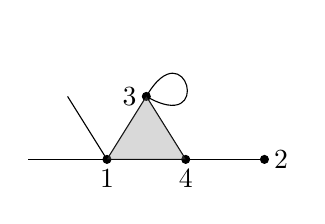
\begin{tikzpicture}
        \tikzset{every loop/.style={min distance=10mm, in=-30, out=60}}
        
        \node [below] at (0,0) {$1$};
	\draw [fill] (0,0) circle [radius=0.05];
        \node [left] at (0.5,0.8) {$3$};
	\draw [fill] (0.5,0.8) circle [radius=0.05];
        \node [below] at (1,0) {$4$};
	\draw [fill] (1,0) circle [radius=0.05];
        \node [right] at (2,0) {$2$};
	\draw [fill] (2,0) circle [radius=0.05];
        \draw (1,0)--(2,0);
        \draw (0,0)--(-1,0);
        \draw (0,0)--(-0.5,0.8);
        \draw (0,0)--(0.5,0.8)--(1,0)--(0,0);
        \draw (0.5,0.8) edge [loop above] node {} (0.5,0.8);
        \fill[gray, opacity=0.3] (0,0)--(1,0)--(0.5,0.8)--(0,0);
    \end{tikzpicture}{\caption{an extended quiver}\label{extquiver}}
\end{figure}

Attached to such an $A$ we also have a representation $V_A$ of $\prod_{a\in X}(\sl_2)_a$. Let $V_1$ be the tautological representation of $\sl_2$ and $V_d=S^dV_1$ for $d\geq 1$. Then, the irreducible components of $V_A$ correspond to elements of $Y$, and are as follows:

\begin{enumerate}
    \item For $a\in Y$: the tautological representation $V_1$ of $(\sl_2)_a$,
    \item For $\{a,a\}\in Y$: the representation $V_2$ of $(\sl_2)_a$,
    \item For $\{a,b\}\in Y$ with $a\neq b$: the representation $V_1\boxtimes V_1$ of $(\sl_2)_a\times(\sl_2)_b$,
    \item For $\{a,b,c\}\in Y$: the representation $V_1\boxtimes V_1\boxtimes V_1$ of $(\sl_2)_a\times(\sl_2)_b\times(\sl_2)_c$.
\end{enumerate}
Note that if there are no triples in $Y$, then this is a framed quiver representation as seen in the theory of quiver varieties (see \cite[Section 3.1]{ginzburg2009lecturesonnakajimaquivervarieties}), where the dimension of the vector space at each vertex is $2$ and the dimension of the framing at each vertex is the multiplicity of that vertex in $Y$. This is the motivation for the name extended quiver, and we will call the corresponding representations \textbf{extended quiver representations}. If $A$ is an extended quiver, let $V(A)$ be the corresponding representation.

We say an extended quiver is of \textbf{trivial type} if it is one of the following (note the recursive definition):

\begin{enumerate}
    \item A single vertex, a vertex with a framing, a path graph with a single framing on each terminal vertex (a path of length $1$ has two framings on the sole vertex), an $l$-cycle (a $1$-cycle is a self-loop), or a $3$-hyperedge,
    \item An extended quiver of trivial type with a leaf attached to one of its vertices,
    \item A disjoint union of extended quivers of trivial type.
\end{enumerate}

For example, the following extended quiver is of trivial type, while the one in Figure \ref{extquiver} is not.

\begin{figure}[H]
    \centering
    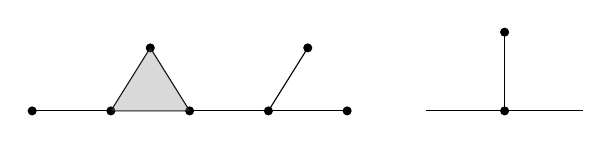
\begin{tikzpicture}
	\draw [fill] (0,0) circle [radius=0.05];
	\draw [fill] (0.5,0.8) circle [radius=0.05];
	\draw [fill] (1,0) circle [radius=0.05];
	\draw [fill] (2,0) circle [radius=0.05];
        \draw [fill] (-1,0) circle [radius=0.05];
        \draw [fill] (3,0) circle [radius=0.05];
        \draw [fill] (2.5,0.8) circle [radius=0.05];
        \draw (1,0)--(2,0)--(3,0);
        \draw (2,0)--(2.5,0.8);
        \draw (0,0)--(-1,0);
        \draw (0,0)--(0.5,0.8)--(1,0)--(0,0);
        \fill[gray, opacity=0.3] (0,0)--(1,0)--(0.5,0.8)--(0,0);

        \draw [fill] (5,0) circle [radius=0.05];
        \draw [fill] (5,1) circle [radius=0.05];
        \draw (4,0)--(6,0);
        \draw (5,0)--(5,1);
    \end{tikzpicture}{\caption{an extended quiver of trivial type}\label{extquivertriv}}
\end{figure}

An extended quiver of trivial type arising from the first part of the definition will be called a \textbf{basic extended quiver}. An extended quiver containing no $l$-cycles is called \textbf{acyclic}.

Analogously, we also say an extended quiver representation is of trivial type if its corresponding extended quiver is of trivial type, and we call the representations corresponding to basic extended quivers \textbf{basic extended quiver representations}.

\begin{lemma}\label{lem:cofree}
    Let $A,A_1,A_2$ be extended quivers of trivial type. Let $A'$ be obtained from $A$ by adding a leaf.
    
    \begin{enumerate}
        \item All basic extended quiver representations are cofree.\label{lem:cofree1}
        \item If $V(A)$ is cofree, then $V(A')$ is cofree.\label{lem:cofree2}
        \item If $V(A_1),V(A_2)$ are cofree, then $V(A_1\sqcup A_2)$ is cofree.\label{lem:cofree3}
    \end{enumerate}
\end{lemma}

\begin{proof}
We prove \ref{lem:cofree2}.~first.

\ref{lem:cofree2}.

Write $V=V(A),V'=V(A')$, and let $V''\cong V_1\boxtimes V_1$ be the representation corresponding to the edge connecting the leaf to $A$, so that $V'=V\oplus V''$. Let $\g'\cong\sl_2$ be the copy of $\sl_2$ corresponding to the leaf. A simple calculation of the dimensions of weight spaces of $\C[V'']_d$ shows that we have
\[\C[V'']_d\cong V_d\boxtimes V_d\oplus V_{d-2}\boxtimes V_{d-2}\oplus V_{d-4}\boxtimes V_{d-4}\oplus\cdots.\]
In particular, irreducible representations in $\C[V'']$ are all of the form $V_i\boxtimes V_i$ for some $i\geq 0$. Now, note that we have a decomposition $\C[V']=\C[V]\otimes\C[V'']$, so any copy of the trivial representation inside $\C[V']$ must be a direct summand of $M\otimes (V_i\boxtimes V_i)$ for some irreducible representation $M$ in $\C[V]$. But since $\g'$ acts trivially on $V$, the action of $\g'$ on $M\otimes (V_i\boxtimes V_i)$ will always be via a direct sum of copies of $V_i$. In particular, for there to be a trivial representation inside $M\otimes (V_i\boxtimes V_i)$ we must have $i=0$. But then we have $M\otimes (V_i\boxtimes V_i)\cong M\otimes\C\cong M$, so we must also have $M\cong\C$. It follows that we have $\C[V']^G=\C[V]^G\otimes\C[V'']^G$.

Note that from the decomposition of $\C[V'']_d$ above we see that $\C[V'']^G$ is a polynomial algebra in one variable in degree 2, so in particular is a PID. Then as a graded torsion-free module with finite-dimensional graded components over a PID, $\C[V'']$ is free, hence $V''$ is cofree. So $\C[V]$ and $\C[V'']$ are free over $\C[V]^G,\C[V'']^G$, respectively, so it follows that $\C[V']=\C[V]\otimes\C[V'']$ is free over $\C[V]^G\otimes\C[V'']^G=\C[V']^G$, so $V'$ is cofree.

\ref{lem:cofree1}.

The single vertex corresponds to the zero representation of $\sl_2$, for which we have $\C[V]^G=\C[V]$. So this is cofree. A vertex with a framing corresponds to the representation $V=V_1$ of $\sl_2$, and it is well-known that $\C[V]$ decomposes as $\C\oplus V_1\oplus V_2\oplus\cdots$ as a representation of $\sl_2$, so $\C[V]^G=\C$ and $V$ is cofree.

For a path of length $l$ with framings on each terminal vertex, let us first compute $\dim_q\C[V]^G$. Let $(V_i)_k$ be the representation on which the $k$-th copy of $\sl_2$ acts by $V_i$ and all other copies of $\sl_2$ act trivially. Then from the proof of Lemma \ref{lem:cofree} \ref{lem:cofree2}.~we have that
\[\ch_q\C[(V_1)_k\otimes(V_1)_{k+1}]=\frac{1}{1-q^2}\sum_{d\geq 0}\ch((V_d)_k\otimes(V_d)_{k+1})q^d.\]
On the other hand we have $\ch_q\C[(V_1)_k]=\sum_{d\geq 0}\ch(V_d)_kq^d$. Note that $V$ is the direct sum of the representations $(V_1)_1,(V_1)_1\otimes (V_1)_2,\dots,(V_1)_{l-1}\otimes (V_1)_l,(V_1)_l$. Then it is clear that for each $d\geq 0$, there is a copy of $\C$ in $\C[V]$ for each representation of the form
\[(V_d)_1\otimes((V_d)_1\otimes(V_d)_2)\otimes\cdots\otimes((V_d)_{l-1}\otimes (V_d)_l)\otimes (V_d)_l\]
inside $\C[(V_1)_1]\otimes\C[(V_1)_1\otimes (V_1)_2]\otimes\cdots$, and that these are the only copies of $\C$ that are in $\C[V]$. It follows that $\C[V]^G$ is freely generated by the generators of $\C[(V_d)_k\otimes(V_d)_{k+1}]^G$ for $1\leq k\leq l-1$ and the lowest degree copy of $\C$ in
\[(V_1)_1\otimes((V_1)_1\otimes(V_1)_2)\otimes\cdots\otimes((V_1)_{l-1}\otimes (V_1)_l)\otimes (V_1)_l.\]

For the $l$-cycle with $l>1$, we have
\[V=\bigoplus_{k=1}^l(V_1)_k\boxtimes(V_1)_{k+1}\]
where we define $(V_1)_{l+1}=(V_1)_1$. A similar computation to the previous case shows that $\C[V]^G$ is freely generated by the generators of $\C[(V_d)_k\otimes(V_d)_{k+1}]^G$ and the lowest copy of $\C$ in
\[((V_1)_1\otimes(V_1)_2)\otimes\cdots\otimes((V_1)_{l-1}\otimes (V_1)_l)\otimes((V_1)_l\otimes(V_1)_1).\]

For the $3$-hyperedge, it was proved in \cite{littelmann} that $V$ is cofree.

\ref{lem:cofree3}.

Let $V_1=V(A_1),V_2=V(A_2),V=V_1\oplus V_2$. Let $\g_1,\g_2$ be the direct sum of all copies of $\sl_2$ corresponding to vertices in $A_1,A_2$, respectively. Then any copy of the trivial representation inside $\C[V]$ is a direct summand of $M_1\otimes M_2$ for some irreducible representations $M_1,M_2$ in $\C[V_1],\C[V_2]$, respectively. But $\g_1$ acts trivially on $M_2$, so if it acts trivially on some summand of $M_1\otimes M_2$ then it must act trivially on $M_1$. Similarly, $\g_2$ must act trivially on $M_2$. It follows that $M_1\cong M_2\cong\C$, so we have $\C[V]^G=\C[V_1]^G\boxtimes\C[V_2]^G$. Then $\C[V]=\C[V_1]\boxtimes\C[V_2]$ is the tensor product of two free modules, hence is free over $\C[V]^G$.
\end{proof}

\begin{lemma}\label{lem:trivtype}
    Let $A,A_1,A_2$ be extended quivers of trivial type. Let $A'$ be obtained from $A$ by adding a leaf.
    
    \begin{enumerate}
        \item All basic extended quiver representations satisfy \eqref{eq:id}.\label{lem:trivtype1}
        \item If $V(A)$ satisfies \eqref{eq:id}, then $V(A')$ satisfies \eqref{eq:id}.\label{lem:trivtype2}
        \item If $V(A_1),V(A_2)$ satisfy \eqref{eq:id}, then $V(A_1\sqcup A_2)$ satisfies \eqref{eq:id}.\label{lem:trivtype3}
    \end{enumerate}
\end{lemma}

\begin{proof}
\ref{lem:trivtype1}.

A single vertex corresponds to the zero representation of $\sl_2$, for which we have $\dim_q\C[V]^G=\dim_q\C[V^{\rho^\vee}]^\h=1$. So we have $X_V=1$ and \eqref{eq:id} becomes $1=1$.

A vertex with framing corresponds to $V=V_1$, for which we have $S_+=\{1\},\dim_q\C[V]^G=1,\dim_q\C[V^{\rho^\vee}]^\h=1$. Borrowing notation from Section \ref{sec:eqdim}, we have $\lambda_{\{1\}}=0$, which lies on a reflection hyperplane. So we are left with $X_V=1$, and \eqref{eq:id} once again becomes $1=1$.

Let $V$ be a path of length $l$ with framings on each terminal vertex. Then from the proof of Lemma \ref{lem:cofree} \ref{lem:cofree1}.~it follows that $\dim_q\C[V]^G=\frac{1}{(1-q^2)^{l-1}(1-q^{l+1})}$.
For the $k$-th copy of $\sl_2$, let its fundamental weight be $\b{e}_k$. Then $S_+$ consists of $\b{e}_1,\b{e}_l$, and $\b{e}_k+\b{e}_{k+1}$ for $1\leq k\leq l-1$ and $S_0$ consists of $\b{e}_k-\b{e}_{k+1},-\b{e}_k+\b{e}_{k+1}$ for $1\leq k\leq l-1$. We then see that $(S_0)_0$ consists of functions on $S_0$ that take the same values on $\b{e}_k-\b{e}_{k+1},-\b{e}_k+\b{e}_{k+1}$ for each $k$, so we obtain $\dim_q\C[V^{\rho^\vee}]^\h=\frac{1}{(1-q^2)^{l-1}}$. From the description of $S_+$ it is also clear that the only $I\neq\varnothing\subset S_+$ for which $\lambda_I$ does not lie on a reflection hyperplane is $I=S_+$, for which we have $\lambda_I=-\sum_{k=1}^l\b{e}_k$. The coefficient this contributes to $X_V$ is $(-1)^l(-q)^{l+1}=-q^{l+1}$, so $X_V$ becomes $1-q^{l+1}$, which is exactly $\frac{\dim_q\C[V^{\rho^\vee}]^\h}{\dim_q\C[V]^G}$.

The $1$-cycle corresponds to the adjoint representation of $\sl_2$, for which we already know \eqref{eq:id} holds.

For the $l$-cycle with $l>1$, the proof of Lemma \ref{lem:cofree} \ref{lem:cofree1}.~shows that $\dim_q\C[V]^G=\frac{1}{(1-q^2)^l(1-q^l)}$. $S_0$ consists of all weights $\b{e}_k-\b{e}_{k+1},-\b{e}_k+\b{e}_{k+1}$ for $k\in\Z/l\Z$. If $v_\mu$ is an element of $V$ in the $\mu$-weight space, $\C[V^{\rho^\vee}]^\h$ is generated by $p_k:=v_{\b{e}_k-\b{e}_{k+1}}v_{-\b{e}_k+\b{e}_{k+1}}$, $p_+:=\prod_{k\in\Z/l\Z}v_{\b{e}_k-\b{e}_{k+1}}$, and $p_-:=\prod_{k\in\Z/l\Z}v_{-\b{e}_k+\b{e}_{k+1}}$, with the relation $p_+p_-=\prod_{k\in\Z/l\Z}p_k$. So we obtain $\dim_q\C[V^{\rho^\vee}]^\h=\frac{1-q^{2l}}{(1-q^2)^l(1-q^l)^2}$. 
We have $S_+=\{\b{e}_k+\b{e}_{k+1}\}$ for $k\in\Z/l\Z$, and again it is easy to see that the only $I\neq\varnothing\subset S_+$ for which $\lambda_I$ does not lie on a reflection hyperplane is $I=S_+$, for which we have $\lambda_I=-\sum_{k\in\Z/l\Z}\b{e}_k$. This contributes the coefficient $(-1)^l(-q)^l=q^l$ to $X_V$, so $X_V$ becomes $1+q^l$, which is exactly $\frac{\dim_q\C[V^{\rho^\vee}]^\h}{\dim_q\C[V]^G}$.

Finally, for the $3$-hyperedge, we have $\dim_q\C[V]^G=\frac{1}{1-q^4}$ from \cite{littelmann}. We also have $S_0=\varnothing$, so $\dim_q\C[V^{\rho^\vee}]^\h=1$. We have $S_+=\{\b{e}_1+\b{e}_2+\b{e}_3,-\b{e}_1+\b{e}_2+\b{e}_3,\b{e}_1-\b{e}_2+\b{e}_3,\b{e}_1+\b{e}_2-\b{e}_3\}$. The $I\neq \varnothing\subset S_+$ for which $\lambda_I$ does not lie on a reflection hyperplane are all 2 and 4 element subsets of $S_+$. A short computation shows that the 2 element subsets cancel out in $X_V$, and the 4 element subset contributes $(-1)^3(-q)^4=-q^4$. So $X_V$ becomes $1-q^4$, which is exactly $\frac{\dim_q\C[V^{\rho^\vee}]^\h}{\dim_q\C[V]^G}$.

\ref{lem:trivtype2}.

Let $V=V(A),V'=V(A')$. Let $V''\cong V_1\boxtimes V_1$ be the summand of $V'$ corresponding to the edge connecting the leaf. From the proof of Lemma \ref{lem:cofree} \ref{lem:cofree2}.~we have that 
\begin{equation*}
\dim_q\C[V']^G=\dim_q\C[V]^G\dim_q\C[V'']^G=\frac{\dim_q\C[V]^G}{(1-q^2)}.
\end{equation*}
Let $\g''\cong\sl_2$ be the copy of $\sl_2$ in the Lie algebra for $A'$ corresponding to the leaf and let $\omega$ be the fundamental weight of $\g''$. We have $S_0=S_0^V\cup S_0^{V''}$, where $S_0^V,S_0^{V''}$ are the sets $S_0$ for $V,V''$, respectively. Note that every element of $S_0^V$ is orthogonal to $\omega$, so the only functions in $(S_0)_0$ must be equal on both elements of $S_0^{V''}$. This implies $\C[(V')^{\rho^\vee}]^\h=\C[V^{\rho^\vee}]^\h\otimes\C[(V'')^{\rho^\vee}]^\h$, so $\dim_q\C[(V')^{\rho^\vee}]^\h=\dim_q\C[V^{\rho^\vee}]^\h\dim_q\C[(V'')^{\rho^\vee}]^\h=\frac{\dim_q\C[V^{\rho^\vee}]^\h}{1-q^2}$. So we have $\frac{\dim_q\C[(V')^{\rho^\vee}]^\h}{\dim_q\C[V']^G}=\frac{\dim_q\C[V^{\rho^\vee}]^\h}{\dim_q\C[V]^G}$.

Let $S_+^V,S_+^{V''}$ be the sets $S_+$ for $V,V''$, respectively. Then we have $S_+=S_+^V\cup S_+^{V''}$, and $S_+^{V''}$ consists of a single element, call it $\alpha'$. Then note that for any $I\subset S_+$, if $\alpha'\in I$ then $\langle\lambda_I,\omega\rangle=0$, so $\lambda_I$ lies on a reflection hyperplane. So the only $I$ that contribute to $X_{V'}$ are subsets of $S_+^V$, and we get $X_V=X_{V'}$. So \eqref{eq:id} holds for $V'$ since it holds for $V$.

\ref{lem:trivtype3}.

Let $V'=V(A_1),V''=V(A_2),V=V(A_1\sqcup A_2)$. Then we have $\C[V]=\C[V']\boxtimes\C[V'']$, so we have $\dim_q\C[V]^G=\dim_q\C[V']^G\dim_q\C[V'']^G$. If $S_+',S_+'',S_0',S_0''$ are the sets $S_+,S_0$ for $V',V''$, respectively, then we have $S_+=S_+'\cup S_+'',S_0=S_0'\cup S_0''$. Moreover, any element of $S_+'$ is always orthogonal to any element of $S_+''$, and the same holds for $S_0',S_0''$. The former implies $X_V=X_{V'}X_{V''}$ and the latter implies $\dim_q\C[V^{\rho^\vee}]^\h=\dim_q\C[(V')^{\rho^\vee}]^\h\dim_q\C[(V'')^{\rho^\vee}]^\h$. So \eqref{eq:id} holds for $V$ since it holds for $V',V''$.
    
\end{proof}

Note that for all extended quiver representations of trivial type containing no $l$-cycles, the proof of Lemma \ref{lem:trivtype} implies that $\C[V^{\rho^\vee}]$ is free over $\C[V^{\rho^\vee}]^\h$. In particular, we obtain

\begin{proposition}\label{prop:sl2s}
    Theorem \ref{thm} holds for all acyclic extended quiver representations of trivial type.
\end{proposition}

Note that taking the direct sum of any representation with the trivial representation does not change any of $\C[\N_V]$, $X_V$, or cofreeness, so Theorem \ref{thm} also holds if we take the direct sum of an acyclic extended quiver representation of trivial type with copies of the trivial representation.

Through computer calculations, we expect Theorem \ref{thm} to hold for all extended quiver representations of trivial type, including ones with $l$-cycles. However, the $l$-cycles have the property that $\C[V^{\rho^\vee}]$ is not free over $\C[V^{\rho^\vee}]^\h$. Indeed, in the proof of Lemma \ref{lem:trivtype} it was shown that $\C[V^{\rho^\vee}]^\h$ is not a free commutative $\C$-algebra, and the statement follows from \cite[Lemma 4.2.10]{springer}. As illustrated by the following, this makes any proof of Theorem \ref{thm} in this case much more complicated.

\begin{proposition}\label{prop:2cycle}
    Theorem \ref{thm} holds for the extended quiver representation corresponding to the $2$-cycle.
\end{proposition}

\begin{proof}
    Let $A=\C[V^{\rho^\vee}]^\h$. By Proposition \ref{prop:hesselink}, we wish to show
    \[\sum_{w\in W}(-1)^{\ell(w)}t^{w\rho}\sum_{\lambda\in\Lambda_+}t^{w\lambda}\M_q(\lambda)=\sum_{w\in W}(-1)^{\ell(w)}t^{w\rho}w\left(\frac{1}{\dim_qA\prod_{\alpha\in S_{\leq 0}}(1-qt^{-\alpha})}\right).\]
    Using the definition of $\M_q$, this is equivalent to
    \[\dim_qA\sum_{w\in W}(-1)^{\ell(w)}t^{w\rho}\sum_{\lambda\in\Lambda}\P_q(w\lambda)t^{w\lambda}=\sum_{w\in W}(-1)^{\ell(w)}t^{w\rho}\left(\frac{1}{\prod_{\alpha\in S_{\leq 0}}(1-qt^{-w\alpha})}\right).\]
    Let $m:S_0\to\Z_{\geq 0}$ be a function. We will use the shorthand $t^m$ to mean $\prod_{\alpha\in S_0}t^{m(\alpha)\alpha}$ and $|m|$ to mean $\sum_{\alpha\in S_0}m(\alpha)$. Also, let $WN(S_0)$ be the set of weakly negative functions on $S_0$. We wish to show that
    \begin{equation}\label{eq:2cycle}
        t^\rho\frac{1}{\prod_{\alpha\in S_-}(1-qt^{-\alpha})}\left(\dim_qA\sum_{m\in WN(S_0)}q^{|m|}t^{-m}-\sum_{m\in\Z_{\geq 0}S_0}q^{|m|}t^{-m}\right).
    \end{equation}
    is zero after antisymmetrization. Note that $\sum_{m\in\Z_{\geq 0}S_0\setminus(S_0)_0}q^{|m|}t^{-m}$ is exactly the $q$-character of the space of generators of $\C[V^{\rho^\vee}]$ as an $A$-module, and thus the part of \eqref{eq:2cycle} in parentheses exactly measures the $q$-character of the syzygies of $\C[V^{\rho^\vee}]$ as an $A$-module.

    Let us compute these syzygies. Weights for $\g=\sl_2\oplus\sl_2$ can be described as ordered pairs of integers, and we have $S_0=\{(1,-1),(1,-1),(-1,1),(-1,1)\}$. Let $a_1,a_2,b_1,b_2$ be the generators of $\C[V^{\rho^\vee}]$ such that the $a_i$ have weight $(1,-1)$ and the $b_i$ have weight $(-1,1)$. Then $A$ is generated by
    \[p_1:=a_1b_1,\quad p_2:=a_1b_2,\quad p_3:=a_2b_1,\quad p_4:=a_2b_2\]
    with the relation $p_1p_4=p_2p_3$. The generators of $\C[V^{\rho^\vee}]$ over $A$ are given by $1$, $e_{d,k}:=a_1^{d-k}a_2^k$ for $d>0,0\leq k\leq d$, and $f_{d,k}:=b_1^{d-k}b_2^k$. 

    For $d\in\Z$, let $\C[V^{\rho^\vee}]_d$ be the $A$-submodule of $\C[V^{\rho^\vee}]$ consisting of elements with weight $(d,-d)$. For $d\geq 0$, the generators of this submodule are $e_{d,k}$ for $0\leq k\leq d$. A resolution of $\C[V^{\rho^\vee}]_d$ is given by
    \[\cdots\xto{\partial_2}A\{f^2_k,g^2_k\}_{0\leq k\leq d-1}\xto{\partial_1}A\{f^1_k,g^1_k\}_{0\leq k\leq d-1}\xto{\partial_0}A\{e_{d,k}\}_{0\leq k\leq d},\]
    where
    \begin{align*}
        \partial_0(f_k^1)&=p_3e_{d,k}-p_1e_{d,k+1},&\partial_0(g_k^1)&=p_4e_{d,k}-p_2e_{d,k+1},\\
        \partial_i(f_k^{i+1})&=p_3f_k^i-p_1g_k^i,&\partial_i(g_k^{i+1})&=p_4f_k^i-p_2g_k^i
    \end{align*}
    if $i>0$ is even, and
    
    \[\partial_i(f_k^{i+1})=p_2f_k^i-p_1g_k^i,\quad\partial_i(g_k^{i+1})=p_4f_k^i-p_3g_k^i\]
    if $i$ is odd. Indeed, a relation $F=0$ for $F\in A\{e_{d,k}\}$ can be assumed homogeneous in its multidegree in $b_1,b_2$. Then a straightforward induction argument shows $F$ can be generated by $\partial_0(f_k^1),\partial_0(g_k^1)$, which are the relations with multidegree $(1,0),(0,1)$, respectively. So $\coker\partial_0=\C[V^{\rho^\vee}]_d$. We have that $\ker\partial_0$ is generated by elements in $A\{f_k^1,g_k^1\}$ for fixed $k$. Indeed, this is clear since given $F\in\ker\partial_0$, we can consider which $e_{d,k}$ appear in $\partial_0(F)$. From there, it is easy to see that $\ker\partial_0$ is generated by $\partial_1(f_k^2),\partial_1(g_k^2)$. The same argument then shows exactness at each $A\{f_k^r,g_k^r\}$.
    
    Thus we obtain
    \begin{align*}
        \dim_q\C[V^{\rho^\vee}]_d&=\dim_qA\left((d+1)q^d-2d(q^{d+2}-q^{d+4}+q^{d+6}-\cdots)\right)\\
        &=\dim_qA\left((d+1)q^d-\frac{2dq^{d+2}}{1+q^2}\right)
    \end{align*}
    where the $(d+1)q^d$ term comes from the generators and the rest of the terms from the syzygies. A similar calculation yields the same result when $d<0$.

    Thus we obtain
    \[\dim_qA\sum_{m\in\Z_{\geq 0}S_0\setminus(S_0)_0}q^{|m|}t^{-m}-\sum_{m\in\Z_{\geq 0}S_0}q^{|m|}t^{-m}=\dim_qA\sum_{d\neq 0}t^{(d,-d)}\left(\frac{2|d|q^{|d|+2}}{1+q^2}\right).\]
    We can write
    \[\sum_{d>0}dt^{(d,-d)}q^{d-1}=\frac{t^{(1,-1)}}{(1-qt^{(1,-1)})^2},\quad\sum_{d>0}dt^{(-d,d)}q^{d-1}=\frac{t^{(-1,1)}}{(1-qt^{(-1,1)})^2},\]
    so \eqref{eq:2cycle} can be written as
    \begin{align*}
        &\frac{2q^3\dim_qA}{1+q^2}\left(\frac{t^{(1,1)}}{(1-qt^{(1,1)})^2}\right)\left(\frac{t^{(1,-1)}}{(1-qt^{(1,-1)})^2}+\frac{t^{(-1,1)}}{(1-qt^{(-1,1)})^2}\right)\\
        =&\frac{2q^3\dim_qA}{1+q^2}\left(\frac{t^{(2,0)}}{(1-qt^{(1,1)})^2(1-qt^{(1,-1)})^2}+\frac{t^{(0,2)}}{(1-qt^{(1,1)})^2(1-qt^{(-1,1)})^2}\right).
    \end{align*}
    The action of the two simple reflections in $W$ on weights are via $(a,b)\mapsto(a,-b)$ and $(a,b)\mapsto(-a,b)$. The two terms in the above are invariant under the former and latter of these, respectively. Thus both terms go to zero after antisymmetrization.
\end{proof}

\begin{remark}\label{rem:resolution}
    The proof of Proposition \ref{prop:2cycle} illustrates a general idea for proving Theorem \ref{thm} using \eqref{eq:id}. Namely, let $A=\C[V^{\rho^\vee}]^\h$, and suppose we have a free resolution of $A$-modules
    \[\cdots\to F_2\to F_1\to F_0\to\C[V^{\rho^\vee}].\]
    Then we obtain $\ch_q\C[V^{\rho^\vee}]=\sum_{i\geq 0}(-1)^i\ch_qF_i$. So following the first paragraph of the proof of Proposition \ref{prop:2cycle}, a proof of Theorem \ref{thm} reduces to a proof that
    \[\sum_{w\in W}(-1)^{\ell(w)}w\left(\frac{t^\rho\sum_{i\geq 1}(-1)^i\ch_qF_i}{\prod_{\alpha\in S_-}(1-qt^{-\alpha})}\right)=0.\]
    Note that if $\C[V^{\rho^\vee}]$ is free over $\C[V^{\rho^\vee}]^\h$, the resolution is trivial, so this is automatically satisfied. This recovers the idea from Section \ref{sec:id} that if $\C[V^{\rho^\vee}]$ is free over $\C[V^{\rho^\vee}]^\h$, then \eqref{eq:id} implies Theorem \ref{thm}.
\end{remark}

\begin{remark}
    If instead of looking at a product of $\sl_2$'s we look at a product of $\gl_2$'s, then we may interpret the $l$-cycle as the representation of a cyclic quiver with equal dimensions, from which we can obtain the original extended quiver representation for $\prod\sl_2$ by pulling back along the inclusion $\prod\sl_2\hookrightarrow\prod\gl_2$. Then Theorem \ref{thm} holds for the $\prod\gl_2$-representations by Section \ref{sec:eqdim}. Indeed, for such representations of a product of $\gl_2$'s we do have the condition that $\C[V^{\rho^\vee}]$ is free over $\C[V^{\rho^\vee}]^\h$, because there are fewer $\h$-invariants for $\prod\gl_2$ than for $\prod\sl_2$.

    In principle, one could prove an analog of Proposition \ref{prop:sl2s} for a product of $\gl_2$'s by creating analogs of all of the extended quiver representations for $\gl_2$. It would be interesting to see whether such an analog could be used to classify representations for $\prod\gl_2$ such that Theorem \ref{thm} holds, or whether there are many more such representations.
\end{remark}

\begin{conjecture}
    Let $\g=\prod\sl_2$. Then $V$ is the direct sum of an extended quiver representation of trivial type and any number of copies of the trivial representation if and only if $V$ is Hesselink-type. Moreover, all Hesselink-type representations of $\g$ satisfy \eqref{eq:id} and Theorem \ref{thm} holds for all such representations.
\end{conjecture}

This conjecture is supported by computer calculations for small $V$ and small $\g$, and would serve as strong evidence for Conjecture \ref{conj:cofree} since it would prove the conjecture in the case $\g=\prod\sl_2$. As further evidence for this conjecture, we prove the conjecture for $\g=\sl_2$.

\begin{proposition}\label{prop:sl2}
    Let $\g=\sl_2$. Then the only Hesselink-type representations are direct sums of extended quiver representations of trivial type and copies of the trivial representation.
\end{proposition}
\begin{proof}
    Let $V$ be a Hesselink-type representation of $\sl_2$, and write
    \[V=\bigoplus_{i\geq 0}V_i^{\oplus m_i}.\]
    For $\sl_2$, any positive weight $a$ in $V$ contributes the term $\chi_{V_{a-2}}$ to the coefficient of $q$ in $X_V$. Since $V$ is Hesselink-type, this must be zero for all $a>2$, so we conclude $m_i=0$ if $i>2$. Modulo copies of the trivial character, the coefficient of $q^2$ in $X_V$ is then equal to $-m_1m_2-{m_2\choose{2}}$. This must be zero since $V$ is Hesselink-type, so at least one of $m_1,m_2$ is zero, and if $m_2\neq 0$ then we must have $m_2=1$. If $m_1\neq 0$, then the top degree part of $X_V$ is $\chi_{V_{m_1-2}}$ if $m_1\geq 2$. We conclude that $m_1\leq 2$, so the only possible values of $m_1,m_2$ are
    \[(m_1,m_2)\in\{(0,0),(1,0),(2,0),(0,1)\}.\]
    These correspond to the empty vertex, vertex with one frame, vertex with two frames, and self-loop, respectively. So modulo trivial summands, $V$ must be an extended quiver representation of trivial type.
\end{proof}

\section{More on Hesselink-type representations}\label{sec:small}

\subsection{Geometric interpretation}

Let us interpret the virtual character $X_V$ geometrically. Note that by the Weyl character formula, $X_V$ is equal to a \emph{virtual} character of $\g$ (with coefficients in $\Z[q]$). Given any $\lambda\in\Lambda$, replacing the $\prod_{\alpha\in S_+}(1-qt^{-w\alpha})$ with $t^{w\lambda}$ in the left hand side yields
\[\frac{\sum_{w\in W}(-1)^{\ell(w)}t^{w\rho}t^{w\lambda}}{\sum_{w\in W}(-1)^{\ell(w)}t^{w\rho}},\]
which is exactly the character $\chi_\lambda$ when $\lambda$ is dominant by the Weyl character formula. To determine what happens when $\lambda$ is not dominant, consider the shifted $W$-action on $\lambda$ given by $w\cdot\lambda=w(\lambda+\rho)-\rho$. It is easy to check that for all $y\in W$, we have
\[\frac{\sum_{w\in W}(-1)^{\ell(w)}t^{w\rho}t^{w\lambda}}{\sum_{w\in W}(-1)^{\ell(w)}t^{w\rho}}=\frac{\sum_{w\in W}(-1)^{\ell(w)}t^{w\rho}(-1)^{\ell(y)}t^{w(y\cdot\lambda)}}{\sum_{w\in W}(-1)^{\ell(w)}t^{w\rho}}.\]
In particular, if $y\cdot\lambda$ is dominant then this is $(-1)^{\ell(y)}\chi_{y\cdot\lambda}$. When there is no such $y$, $\rho+\lambda$ is not regular (i.e.~lies on a hyperplane $\langle\alpha,\rho+\lambda\rangle=0$ for some $\alpha\in R_+$), and thus we have
\[\frac{\sum_{w\in W}(-1)^{\ell(w)}t^{w\rho}t^{w\lambda}}{\sum_{w\in W}(-1)^{\ell(w)}t^{w\rho}}=0\]
since the numerator is $W$-antiinvariant and consists of nonregular weights. 

Using this, we can reinterpret the original expression using Borel-Weil-Bott. Namely, let $B\subset G$ be the Borel corresponding to our choice of Cartan subalgebra and polarization, and let $T\subset B$ be its maximal torus. Let $V_+\subset V$ be the direct sum of all weight spaces with weights in $S_+$, which has a structure as a $T$-module and hence as a $B$-module via the quotient map $B\to T$. Note that as a $B$-module, the space $\wedge^\bullet V_+^*$ has $q$-character given exactly by $\prod_{\alpha\in S_+}(1-qt^{-\alpha})$, where the degree in $q$ corresponds to the natural grading on an exterior algebra. Thus by Borel-Weil-Bott, $X_V$ is the $q$-character of
\[R\Gamma(G\times^B(\wedge^\bullet V_+^*))^\vee,\]
where we view $G\times^B(\wedge^\bullet V_+^*)$ as a vector bundle on the flag variety $G/B$ and the $q$-grading is via the grading on the exterior algebra as before. Here, when we take the $q$-character of a derived $G$-module $X_\bullet$ we mean
\[\sum_{i\in\Z}(-1)^i\ch_qH^i(X_\bullet).\]
As the dual of the trivial module is still the trivial module, we obtain
\begin{lemma}
    $V$ is Hesselink-type if and only if $[R\Gamma(G\times^B(\wedge^\bullet V_+^*))]\in\Z[q][\C]$ in the Grothendieck group $K_0(D\mathrm{Rep}(G))[q]$.
\end{lemma}

\subsection{Counterexamples}\label{sec:counter}

As Hesselink-type representations are a new concept and rather mysterious, it is interesting to consider how they might relate to other classes of representations. The first obvious example is whether they have a relation with cofree representations, which is the content of Conjecture \ref{conj:cofree}. We provide some counterexamples to other potential relations one may ask about.

\begin{example}
    Let $\g=\sl_2$, and $V=V_3$ be the irreducible representation with highest weight 3. Then $V$ is cofree\footnote{see \cite{littelmann}, this is also indirectly proved in \cite{vinberg} since the unique outer grading on $\sl_3$ yields $\g_0\cong\sl_2,\g_1\cong V_3$.} and we have $\rho=\rho^\vee=1,W=S_2,S_+=\{1,3\}$. The numerator of $X_V$ becomes $-q^2t^3+qt^2+t-t^{-1}-qt^{-2}+q^2t^{-3}$, whereas if $V$ was Hesselink-type then $X_V$ would have to lie in $(t-t^{-1})\Z[q]$. So not all cofree representations are Hesselink-type.
\end{example}

\begin{example}\label{eg:g2}
    Let $\tilde{\g}$ be a Lie algebra of type $G_2$ with simple roots $\alpha_1,\alpha_2$ where $\alpha_1$ is the long root and $\alpha_2$ is the short root. For $i=0,1$, let $\g_i$ be the direct sum of all weight spaces of $\tilde{\g}$ with weight $\lambda$ such that $\langle\lambda,\alpha_1^\vee\rangle\equiv i\pmod 2$. Then $\g_0,\g_1$ define an inner grading on $\tilde{\g}$. Let $\g=\g_0,V=\g_1$. Then we have $\g\cong\sl_2\times\sl_2, V\cong V_1\boxtimes V_3$. We have $S_+=\{(1,3),(-1,3),(1,1)\}$, so in particular we have $X_V=1+q\chi_{V_1\boxtimes V_1}-q^2\chi_{V_0\boxtimes V_4}$, so $V$ is not Hesselink-type. So a representation arising from a graded Lie algebra with inner grading is not necessarily Hesselink-type.
\end{example}

\begin{example}\label{eg:3232}
    As mentioned in Remark \ref{rem:>2}, consider the representation $V$ of the cyclic quiver with 4 vertices that has dimension vector $3,2,3,2$. As pointed out in the remark, the numerator of $X_V$ contains terms whose weights do not lie on a reflection hyperplane and are also not in $W\rho$. This is not possible if $X_V$ is a direct sum of trivial characters, so $V$ is not Hesselink-type. So not all representations of cyclic quivers are Hesselink-type.
\end{example}

\printbibliography

\footnotesize{
{\bf V.K.}: Department of Mathematics Harvard University and CMSA, 1 Oxford St, Cambridge, MA 02138, USA\\
\hphantom{x}\quad\, {\tt vkrylov@math.harvard.edu}, {\tt krylovasya@gmail.com}

{\bf F.W.}: Department of Mathematics, MIT,
77 Massachusetts Ave, Cambridge, MA 02139, USA\\
\hphantom{x}\quad\, {\tt fw0@mit.edu}}

\end{document}